%%================================================
%% Filename: chap01.tex
%% Encoding: UTF-8
%% Author: Yuan Xiaoshuai - yxshuai@gmail.com
%% Created: 2012-04-27 15:05
%% Last modified: 2016-08-28 21:07
%%================================================
\chapter{第一章 绪论}
\label{cha:overview}

\section{课题研究的背景}
\label{sec:requirements}

目前国内大学社团的现状与水平

从60年代,中国开始改革开放之后,再到79年人人可以通过考试进入大学。以至现如今,普遍的9年义务教育的时代。大学似乎是国内学生统一的接受知识的环境,这样的环境也同时让社团快速成长起来,以至于大学生参加社团活动成了其密不可分的组成。在这几十年里,大学生社团的管理也从分散逐渐走向严格,有序。管理好一个社团,成了每个社团的重中之重。

同时,有些不规范的管理方案,或者当前的管理方案没有很好的继承下去,下一年的社团必将经历一次重创。人员流失,人心涣散,整个社团死气沉沉,必不会是一个好社团继续发展的氛围。

良好的管理能带给社团活力,成员信息不会丢失,处理事务高效无误,将其他时间真正花在社团发展建设上去。新时期的高校大学生,价值观,世界观趋于多元化,如今的社团管理方式,在现社团上的管理效果甚微,如何去利用如今的信息化技术,科学化的管理社团人员,避免出现重复的劳力,脑力,让社团人员拥有更多的动力去开创新的领域实在是迫在眉睫的任务。

\section{课题研究的意义}
\label{sec:requirements}

本课题先是通过文献研究,了解了国内社团部分出现崩塌,难以管理的现状,个人认为在科学管理方面,可以通过自身学习的计算机知识去开创一种方便的,高效的,简易的网站管理人员制度。这种想法正好可以与其他有关管理社团的想法,比如如何加强社团人员培养,人员交流方面,促进发展等等结合起来,共同形成统一,又自由化的制度体系。这样不仅让每个社团保留自己的个性,同样在未知领域有其他方案可以参考。构成新时期社团优秀的管理模式体系。

相较于传统的社团管理,工具化管理社团带来了多方面的创新:

\begin{itemize}
  \item 人员信息管理的变革。从之前的手动填写到现在的线上线下填写,并以电子方式的保存
  \item 值班表制定的改变。利用计算机编程算法,自动计算每节课人员的安排情况
  \item 社团课下学习的改变。使用线上统计的方式,方便地查看人员学习状况,促进成员学习
  \item 通知活动人员的方式改变。从以前的每条短信人员编辑群发,到利用大公司的可靠 API 一键群发短信与邮件(有必要的话)
\end{itemize}

\section{课题研究的目标}
\label{sec:requirements}

利用自己在大学中所学的知识,完成对社团管理系统的开发,实现如下目标:
\begin{itemize}
  \item 整体系统简易,对于学生几分钟就能够学会
  \item 因为系统为分离式,所以每套系统都有各自的信息的导入导出功能
\end{itemize}
大致系统包含如下:
\begin{itemize}
  \item 报名系统——用于招新活动或比赛活动的报名,包括报名者信息填写、管理员信息收集等
  \item 考核系统——用于人员选拔的水平初试、学习效果检测等
  \item 通知系统——用于短信通知,如会议、面试等的通知
  \item 学习系统——沟通与学习的平台,用于学习经验交流、生活心得体会、学习总结、学习笔记、学习进度等的记录,同时推送感兴趣或热门学习方向等
  \item 值班系统——用于安排成员监管活动的小工具
  \item 最后通过 Docker 工具进行快速的部署
\end{itemize}

\section{网站开发的发展于现状}
\label{sec:requirements}

\subsection{全栈的概念}
\label{sec:requirements}

全栈大多指的是全栈工程师,英文 Full Stack。指的是掌握多种开发调试等技能,并能利用这些技术独立完成产品的人。他们大多以网站开发为主,不仅对前端页面的设计与开发,也会后端接口的实现,更深层次的就是将网站内容搬移到 iOS 与 Android 等平台的 APP 上,实现狭义上的全栈开发。如果说到广义,那就还要加上产品的运维,调试,测试等等,甚至产品的宣传。

可以说,一个全栈工程师在公司里可以凭借一己之力,有效减少公司内部的沟通成本,人员的招聘成本。可以扛起这个部门系统架构,当公司业务调整的时候,每个方向的人力都可以做到有效的补充。

\subsection{前端与后端的融合}
\label{sec:requirements}

说到前后的融合,这就不得不说到前端的一些历史,早在二十年前,前端并不存在,那时候网站开发,无论是功能还是界面设计都是由后端人员独自包揽。到后来,FLASH 可以用来做动画,用 Firework 切图,总之 Web 1.0 时代的网站建设两者并没有很好分离,使得工作流程十分混乱。但是随着 Web 2.0 的到来,网站内容越来越多,前后端逐渐分离,伴随而来的就是 JavaScript 再次的爆发性的发展,前端专注于与用户的交互,而后端则是专注数据的传输,服务的稳定提供。通过Restful API 等一些新兴协议,接口的定义更加规范,HTTP 传输的内容不再冗余。从此,前端开始出现了一些基于 JavaScript 的框架,如React, Angular 和 Vue 等,后端则更加复杂,加入了 Node 中间层对大量 API 请求进行分发,真正的后端处理安全性,可靠性与逻辑性,确保数据上的绝对安全。

\subsection{前端的趋势}
\label{sec:requirements}

在之前讲了前端的来源,相信前端以后的路也十分好走。这一切都归功于 JavaScript 十年以来快速的发展,和 HTML5 的标准发布。2014年,第五代 HTML 标准发布。H5 是由浏览器厂商主导,与 W3C 合作制定的一整套 Web 应用规范,至今仍在不断补充新的草案。我们可以清晰的感受到这一系列规范背后隐含的领导者的勃勃雄心:占领所有屏幕。

从2010年开始出现的 Backbone、Angular.js 等前端 JavaScript 框架的出现。前端开始火了起来。

充分发挥 JavaScript 的本身优势,减少页面的重复刷新,只通过少量数据的更新来更新交互界面的数据。以 MVC,甚至之后更加流行的 MVVC 架构的前端框架支撑起了相当可靠的 SPA (Single Page Application,单页应用)。

以后的趋势也显现出来,一方面 React Native 等一系列框架入侵 Android 与 iOS 等原生 APP 之中,使一个模子的代码可以用在多种客户端中。另一方面 Hybird APP 的诞生,使得想 Weex 阿里的一站式框架得以发展,让 APP 的更新不再依赖每次应用商店的审核,而是通过内置的应用浏览器,对页面进行定期更新。常见的如:淘宝,天猫,京东,QQ等活动页,直接采用的是一些 H5 小页面。

\subsection{后端的趋势}
\label{sec:requirements}

相较于前端,后端的任务则变得更为简单了一些。

\begin{figure}[htbp]
\centering
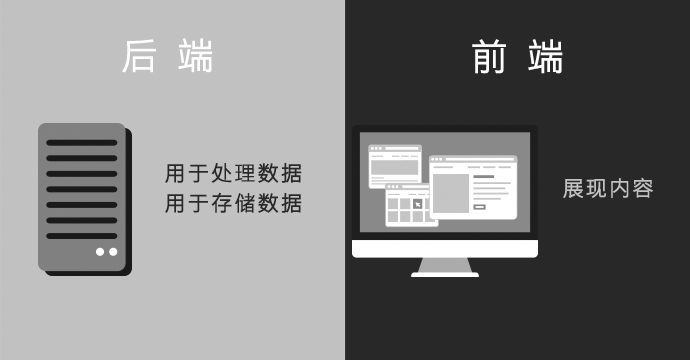
\includegraphics[width=1\textwidth]{02-01-frontend}
\caption{前后端理解}
\label{fig:02-01-frontend}
\end{figure}

互联网发展的早期,前端代码只是后端代码的一部分,大致流程如下:

\begin{itemize}
  \item 后端收到浏览器请求
  \item 生成静态页面
  \item 发送到浏览器
\end{itemize}

那时开发网站,一般采用的都是后端 MVC 模式

\begin{itemize}
  \item Model(模型层):提供/保存数据
  \item Controller(控制层):数据处理,实现业务逻辑
  \item View(视图层):展示数据,提供用户界面
\end{itemize}

前端只是后端 MVC 的 V。以 PHP 框架 Laravel 为例。

\begin{figure}[htbp]
\centering
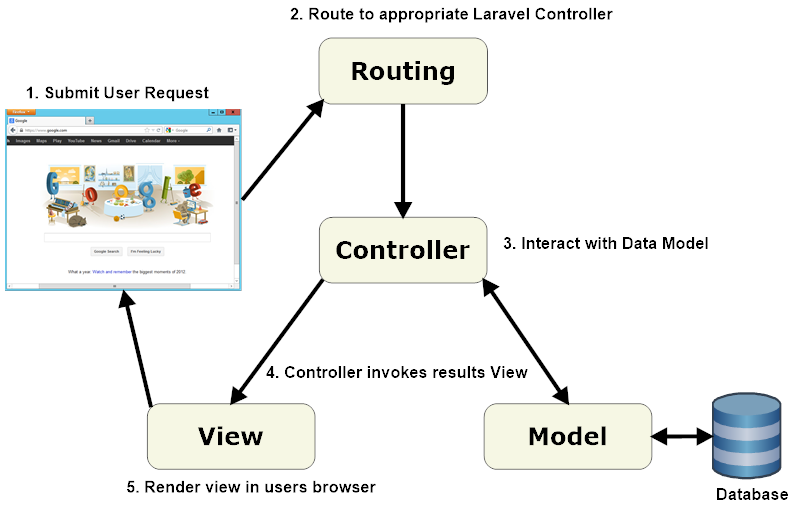
\includegraphics[width=1\textwidth]{02-02-laravel-mvc}
\caption{后端 MVC 中的 View 前端视图}
\label{fig:02-02-laravel-mvc}
\end{figure}

由于 Ajax 技术的广泛应用,前端的应用终于可以独立出来,它们通过异步的请求获取少量数据,这些技术一开始广泛的应用于网页地图上。再到后来,乔布斯发布智能手机开始,很多人都意识到,这种异步获取数据能应用于许多领域上,比如 APP 数据的获取等等。

这两个原因,导师前端开发方式发生了根本的变化,前端不再是后端 MVC 中的 V,而是单独的一层。

前后端分离以后,他们之间通过接口通信进行双向数据传输。后端暴露出接口,前端消费后端提供的数据。后端接口一般是 REST 形式,前后端的通信协议一般是 HTTP。

同时,Node 在2009年诞生,这也就意味着本来只能跑在浏览器的 JavaScript 语言可以同样运行在服务器上,其中最大的意义就是前端工程师可以编写后端程序了。于是,前端工程师正慢慢转变为全栈工程师,一个人负责开发前端与后端,从数据库到 UI 的所有开发。

\subsection{Docker 集装箱模式的盛行}
\label{sec:requirements}

软件开发最大的麻烦事之一就是环境配置。开发环境与部署环境的环境不同,你怎么知道自家的软件,能在哪些机器跑起来?所以开发者必须知道两件事,操作系统是如何设置的,各种第三方库和组件要如何安装。只有当他们都被正确的运行起来,你所开发的程序才能如你所望的跑起来。举个例子,安装一个 Node 应用,计算机必须有 Node 引擎,还必须有各种依赖,可能还要配置环境变量。如果某些老旧的模块与当前环境不兼容,那就麻烦了。开发者常常会说:"它在我的机器可以跑了"(It works on my machine),言下之意就是,其他机器很可能跑不了。环境配置如此麻烦,换一台机器,就要重来一次,旷日费时。很多人想到,能不能从根本上解决问题,软件可以带环境安装?也就是说,安装的时候,把原始环境一模一样地复制过来。

\subsubsection{虚拟机}

虚拟机(virtual machine)就是带环境安装的一种解决方案。它可以在一种操作系统里面运行另一种操作系统,比如在 Windows 系统里面运行 Linux 系统。应用程序对此毫无感知,因为虚拟机看上去跟真实系统一模一样,而对于底层系统来说,虚拟机就是一个普通文件,不需要了就删掉,对其他部分毫无影响。

虽然用户可以通过虚拟机还原软件的原始环境。但是,这个方案有几个缺点。

\begin{itemize}
  \item 资源占用多。虚拟机会独占一部分内存和硬盘空间。它运行的时候,其他程序就不能使用这些资源了。哪怕虚拟机里面的应用程序,真正使用的内存只有 1MB,虚拟机依然需要几百 MB 的内存才能运行。
  \item 冗余步骤多。虚拟机是完整的操作系统,一些系统级别的操作步骤,往往无法跳过,比如用户登录。
  \item 启动慢。启动操作系统需要多久,启动虚拟机就需要多久。可能要等几分钟,应用程序才能真正运行。
\end{itemize}

\subsubsection{Docker}

Docker 属于 Linux 容器的一种封装,提供简单易用的容器使用接口。它是目前最流行的 Linux 容器解决方案。

Docker 将应用程序与该程序的依赖,打包在一个文件里面。运行这个文件,就会生成一个虚拟容器。程序在这个虚拟容器里运行,就好像在真实的物理机上运行一样。有了 Docker,就不用担心环境问题。

总体来说,Docker 的接口相当简单,用户可以方便地创建和使用容器,把自己的应用放入容器。容器还可以进行版本管理、复制、分享、修改,就像管理普通的代码一样。

Docker 的主要用途,目前有三大类。
\begin{itemize}
\item 提供一次性的环境。比如,本地测试他人的软件、持续集成的时候提供单元测试和构建的环境。
\item 提供弹性的云服务。因为 Docker 容器可以随开随关,很适合动态扩容和缩容。
\item 组建微服务架构。通过多个容器,一台机器可以跑多个服务,因此在本机就可以模拟出微服务架构。
\end{itemize}
